\subsection{Brugeradministration}
\label{sub:Brugeradministration}

Brugeradministrationsmodulet har til opgave at kommunikere brugerdata mellem brugeren og databasen.

\subsubsection{Funktionalitet}
\label{ssub:Brugeradministration_funktionalitet}

Kommunikation mellem databasen og brugeren indebærer visning af information omkring en bruger, modtage inputs fra brugeren samt læse fra og skrive i databasen. At læse fra databasen indebærer, at den relevante information bliver hentet fra databasen, og vist på en acceptabel måde. Når der skrives til databasen menes der, at brugerens input bliver gemt i databasen.

\subsubsection{Implementation}
\label{ssub:Brugeradministration_implementation}

\begin{figure}
  \centering
  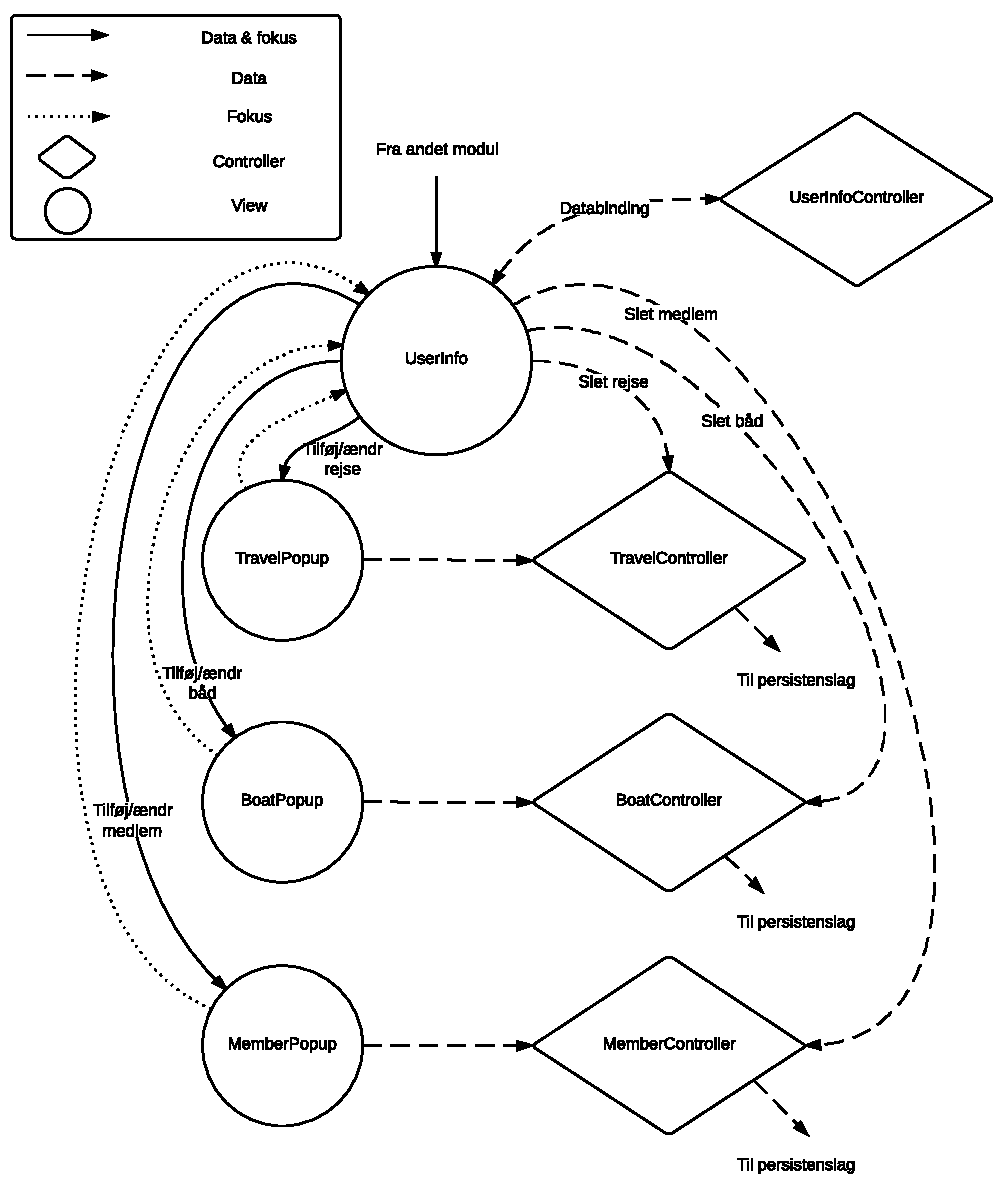
\includegraphics[width=\textwidth]{brugeradministration-diagram.pdf}
  \caption{Diagram over brugeradministrationsmodulet} \label{fig:brugermod}
\end{figure}

For at implementere dette, består brugeradministrationsmodulet af et UserInfo-view, en UserInfoController, samt tre \enquote{popups} med tilhørende \enquote{controllers}. Se \cref{fig:brugermod}. UserInfo-view kan tilgås fra funktionsstyringsmodulet. Denne tilgang kan udføres ved at skifte faneblad, hvorved der ikke sker en ændring af information. Hvis UserInfo-view derimod tilgås vis \enquote{SelectUser}, da ændres informationen til den givne bruger. Se \cref{ssub:hovedmodul_implementation} for mere information.

UserInfoController er ansvarlig for databinding, af den bruger som UserInfo-view fremviser.

Popups'ne og controllerne har parvis deres tilsvarende ansvarsområde, som de sammen står for at håndtere. De tre ansvarsområder er bruger, både og rejser. Popup'en modtager brugerens input, ved tilføjelser og ændringer, og videresender det til dens respektive controller. Controlleren kommunikerer med persistenslaget, som dernæst udfører brugerens ønskede handling. Sletning af brugere, både eller rejser, sker direkte fra UserInfo-view til den respektive controller.

Brugen af popup vinduer, hjælper brugeren med at skelne i mellem læsning og skrivning af data.
